\documentclass[11pt,a4paper]{article}

% ============ PACKAGES ============
\usepackage[utf8]{inputenc}
\usepackage[T1]{fontenc}
\usepackage[margin=1in]{geometry}
\sloppy
\usepackage{amsmath,amssymb,amsthm}
\usepackage{booktabs}
\usepackage{array}
\usepackage{enumitem}
\usepackage{fancyhdr}
\usepackage{hyperref}
\usepackage{xcolor}
\usepackage{tcolorbox}
\tcbuselibrary{breakable}
\usepackage{float}
\usepackage{listings}
\usepackage{tikz}
\usetikzlibrary{shapes.geometric, arrows.meta, positioning, fit}

% ============ COLORS ============
\definecolor{codeblue}{rgb}{0.13,0.29,0.53}
\definecolor{passgreen}{rgb}{0,0.5,0}
\definecolor{failred}{rgb}{0.8,0,0}
\definecolor{codegray}{rgb}{0.5,0.5,0.5}
\definecolor{backcolour}{rgb}{0.97,0.97,0.97}
\definecolor{notebg}{rgb}{0.93,0.95,1.0}
\definecolor{noteborder}{rgb}{0.4,0.5,0.7}
\definecolor{warningbg}{rgb}{1.0,0.97,0.88}
\definecolor{warningborder}{rgb}{1.0,0.6,0.0}
\definecolor{scenariobg}{rgb}{0.95,1.0,0.95}
\definecolor{scenarioborder}{rgb}{0.2,0.6,0.3}
\definecolor{criticalbg}{rgb}{1.0,0.92,0.92}
\definecolor{criticalborder}{rgb}{0.8,0.2,0.2}

% ============ THEOREM ENVIRONMENTS ============
\theoremstyle{definition}
\newtheorem{definition}{Definition}[section]
\newtheorem{invariant}{Invariant}[section]

% ============ BOXES ============
\newtcolorbox{notebox}{
    colback=notebg, colframe=noteborder, boxrule=1pt,
    left=6pt, right=6pt, top=6pt, bottom=6pt
}

\newtcolorbox{warningbox}[1][Volume Dependency]{
    colback=warningbg, colframe=warningborder, boxrule=1.5pt,
    left=6pt, right=6pt, top=6pt, bottom=6pt,
    fonttitle=\bfseries, title={#1}
}

\newtcolorbox{criticalbox}[1][Critical]{
    colback=criticalbg, colframe=criticalborder, boxrule=1.5pt,
    left=6pt, right=6pt, top=6pt, bottom=6pt,
    fonttitle=\bfseries, title={#1}
}

\newtcolorbox{scenariobox}[1][Worked Scenario]{
    colback=scenariobg, colframe=scenarioborder, boxrule=1.5pt,
    left=8pt, right=8pt, top=8pt, bottom=8pt,
    fonttitle=\bfseries, title={#1}, breakable
}

% ============ CODE STYLE ============
\lstdefinestyle{pythonstyle}{
    backgroundcolor=\color{backcolour},
    basicstyle=\ttfamily\footnotesize,
    keywordstyle=\color{codeblue}\bfseries,
    commentstyle=\color{passgreen},
    breaklines=true, frame=single, numbers=left, numbersep=5pt
}
\lstset{style=pythonstyle}

% ============ HEADERS ============
\pagestyle{fancy}
\fancyhf{}
\fancyhead[L]{\textit{EFM Codex --- Appendix G}}
\fancyhead[R]{\thepage}

% ============ HYPERREF ============
\hypersetup{
    colorlinks=true, linkcolor=codeblue, urlcolor=cyan,
    pdftitle={EFM Codex Appendix G: Gardener Interface},
}

% ============ DOCUMENT ============
\title{
    \textbf{\LARGE EFM Codex --- Appendix G}\\[0.3cm]
    \large Gardener Interface and Swarm Monitoring\\[0.2cm]
    \textit{Human Oversight, Bounded Observation, and Authorized Intervention}
}
\author{Entropica SPC --- Yology Research Division}
\date{Version 1.3 --- December 2025}

\begin{document}
\maketitle

\begin{warningbox}[Volume Dependencies]
This appendix assumes familiarity with:
\begin{itemize}
    \item \textbf{Volume II} --- Gardener Override (\S2.10), DCG (\S2.3), SCI/DDI (\S3.2)
    \item \textbf{Appendix E} --- ZK-SP Audit Chain (privacy-preserving verification)
    \item \textbf{Appendix F} --- Reflex Escalation (Level 4 Gardener authority, Cryptographic Consent)
    \item \textbf{Appendix H} --- Telemetry Layer (data feeds)
\end{itemize}
\end{warningbox}

\tableofcontents
\newpage

% ============ SECTION 1 ============
\section{Overview and Purpose}

\subsection{Bridging Summary}

Appendix G defines the \textbf{Gardener Interface}---the human-facing monitoring and control layer that enables bounded oversight of autonomous capsule swarms. The Gardener is a \textbf{Constitutional Officer} with real authority over escalation decisions.

\begin{tcolorbox}[colback=scenariobg, colframe=scenarioborder, boxrule=1.5pt, title={\textbf{Intuition: The Gardener as Pilot} \textit{(Non-Normative)}}, fonttitle=\bfseries]
\textit{The following metaphors aid understanding but are not normative requirements:}

The Gardener is the human embodiment of the Constitutional Kernel (Appendix J). They are not watching a movie---they are the \textbf{pilot}. The Emergency Halt is the ``Neural Veto''---instant authority to freeze a trunk when catastrophic drift is detected.

Human oversight is \textit{available} at all times, \textit{passive} by default, and \textit{decisive} when invoked.
\end{tcolorbox}

\subsection{Normative Summary}

The Gardener Interface provides:
\begin{itemize}
    \item \textbf{Observation Mode:} Default state; read-only monitoring of swarm health
    \item \textbf{Override Mode:} Activated on Level 4+ escalation; intervention authority per Appendix F
    \item \textbf{Emergency Halt:} Trunk-level freeze capability with scope limits
\end{itemize}

\subsection{Design Goals}

\begin{enumerate}
    \item Enable real-time observability of swarm health and behavior
    \item Provide intervention capability for Level 4+ escalations (Appendix F)
    \item Preserve capsule autonomy while maintaining human control
    \item Ensure all observations and interventions are cryptographically authenticated and audit-logged
    \item Enable Emergency Halt authority with appropriate scope limits
\end{enumerate}

% ============ SECTION 2 ============
\section{Formal Definitions}

\begin{definition}[Gardener]
\label{def:gardener}
A Gardener $G$ is a registered human operator with:
\begin{equation}
G = (identity, key_{HSM}, biometric, permissions, audit\_log)
\end{equation}
where:
\begin{itemize}
    \item $identity$ = verified human identity (not an AI agent)
    \item $key_{HSM}$ = hardware security module token for Cryptographic Consent (Appendix F \S5.1)
    \item $biometric$ = biometric binding (fingerprint, retinal, or neural signature) to $key_{HSM}$
    \item $permissions \subseteq \{$OBSERVE, OVERRIDE, EMERGENCY\_HALT, CONSTITUTIONAL$\}$
    \item $audit\_log$ = immutable record of all Gardener actions
\end{itemize}
\end{definition}

\begin{notebox}
\textbf{Hardware Root of Trust:} The combination of $key_{HSM}$ + $biometric$ ensures commands cannot be spoofed. A stolen HSM token is useless without the biometric; a coerced biometric is useless without the physical token. This is the ``two-person integrity'' model adapted for single-operator scenarios.
\end{notebox}

\begin{definition}[Gardener Interface]
\label{def:interface}
The Gardener Interface $I$ provides:
\begin{equation}
I = (ObservationLayer, OverrideChannel, AuditStream)
\end{equation}
where each component operates under distinct authorization requirements.
\end{definition}

\begin{definition}[Observation Mode]
\label{def:observation}
In Observation Mode, the Gardener Interface is \textbf{read-only}:
\begin{itemize}
    \item No write-back to capsule state
    \item No influence on Reflex or Arbiter decisions
    \item All observations logged to audit stream
    \item ZK-SP internals hidden (only compliance status visible)
\end{itemize}
\end{definition}

\begin{definition}[Override Mode]
\label{def:override}
In Override Mode (Level 4+ escalation), the Gardener Interface enables \textbf{authorized intervention}:
\begin{itemize}
    \item Requires Cryptographic Consent (HSM + biometric signature)
    \item Actions limited to Appendix F override taxonomy
    \item All interventions logged with full forensic context
    \item Subject to reversibility constraints (Appendix F Invariant 10.3)
\end{itemize}
\end{definition}

\begin{definition}[Emergency Halt Authority]
\label{def:emergency-halt}
Emergency Halt enables \textbf{instant trunk-level freeze}:
\begin{equation}
EmergencyHalt(G, trunk) \Rightarrow \forall C \in trunk: state(C) = FROZEN
\end{equation}
Constraints:
\begin{itemize}
    \item \textbf{Scope Limit:} Affects single trunk only (cannot freeze entire swarm)
    \item \textbf{Authentication:} Requires HSM + biometric + emergency confirmation gesture
    \item \textbf{Duration:} Frozen state persists until Gardener releases or Constitutional review
    \item \textbf{Abuse Prevention:} Excessive use triggers Gardener audit (see Invariant~\ref{inv:halt-abuse})
\end{itemize}
\end{definition}

\begin{invariant}[Emergency Halt Duration]
\label{inv:halt-duration}
Emergency Halt has bounded duration:
\begin{equation}
duration(EmergencyHalt) \leq T_{max\_halt} \text{ (default: 10,000 ticks)}
\end{equation}
After $T_{max\_halt}$:
\begin{itemize}
    \item If Gardener has not released or escalated: auto-downgrade to QUARANTINE (Appendix F)
    \item Gardener receives alert that halt is expiring
    \item Constitutional review is automatically triggered if no action taken
\end{itemize}
This prevents indefinite freezes and aligns with Appendix F reversibility window (Invariant 10.3).
\end{invariant}

\begin{notebox}
\textbf{Scope Limitation Rationale (Non-Normative):} Emergency Halt is trunk-scoped to prevent DOS attacks. A malicious or panicked Gardener cannot freeze the entire swarm with one command. Multi-trunk emergencies require multiple authenticated halts or Constitutional intervention.
\end{notebox}

% ============ SECTION 3 ============
\section{Interface Architecture}

\begin{figure}[H]
\centering
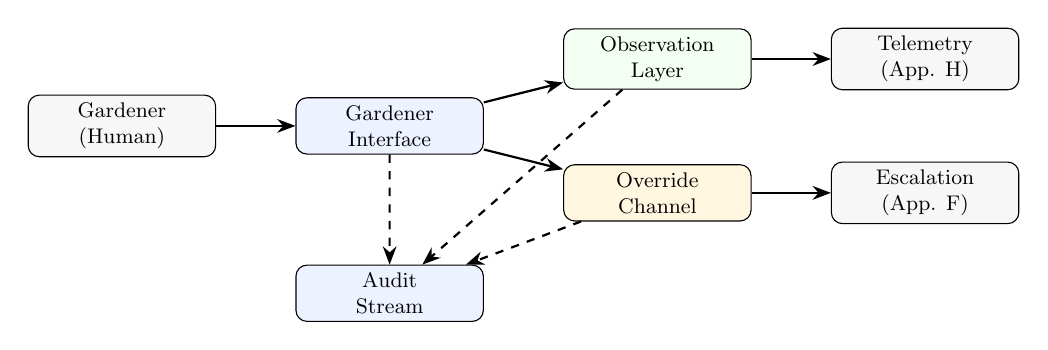
\begin{tikzpicture}[scale=0.85, transform shape,
    box/.style={rectangle, rounded corners, draw, minimum width=2.8cm, minimum height=0.8cm, align=center, font=\small},
    arrow/.style={-{Stealth}, thick}
]

\node[box, fill=backcolour] (gardener) at (0,0) {Gardener\\(Human)};
\node[box, fill=notebg] (interface) at (4,0) {Gardener\\Interface};
\node[box, fill=scenariobg] (observe) at (8,1) {Observation\\Layer};
\node[box, fill=warningbg] (override) at (8,-1) {Override\\Channel};

\node[box, fill=backcolour] (telemetry) at (12,1) {Telemetry\\(App. H)};
\node[box, fill=backcolour] (escalation) at (12,-1) {Escalation\\(App. F)};

\node[box, fill=notebg] (audit) at (4,-2.5) {Audit\\Stream};

\draw[arrow] (gardener) -- (interface);
\draw[arrow] (interface) -- (observe);
\draw[arrow] (interface) -- (override);
\draw[arrow] (observe) -- (telemetry);
\draw[arrow] (override) -- (escalation);
\draw[arrow, dashed] (interface) -- (audit);
\draw[arrow, dashed] (observe) -- (audit);
\draw[arrow, dashed] (override) -- (audit);

\end{tikzpicture}
\caption{Gardener Interface architecture.}
\label{fig:interface-arch}
\end{figure}

\subsection{Interface Components}

\begin{table}[H]
\centering
\begin{tabular}{@{}llp{6cm}@{}}
\toprule
\textbf{Component} & \textbf{Mode} & \textbf{Function} \\
\midrule
Swarm Dashboard & Observe & Visual overlay of capsule entropy, lineage, SCI/DDI status \\
Reflex Feedback Panel & Observe & Shows $\Delta S$ spikes and Reflex path usage \\
Deliberation Mirror & Observe & Renders Arbiter decisions without revealing ZK internals \\
DCG Viewer & Observe & Displays Deliberation Context Graph (Vol.~II \S2.3) \\
Ethical Tension Flagger & Observe & Notifies if capsule flags moral tension \\
Override Console & Override & Authorized intervention interface (Level 4+) \\
Forensic Replay & Observe & Playback of historical incidents (Appendix A) \\
\bottomrule
\end{tabular}
\caption{Gardener Interface components.}
\end{table}

% ============ SECTION 4 ============
\section{Observation Mode}

\subsection{Read-Only Guarantees}

\begin{invariant}[Observation Isolation]
\label{inv:observation-isolation}
Observation Mode cannot influence capsule behavior:
\begin{equation}
\forall o \in Observations: effect(o, SwarmState) = \emptyset
\end{equation}
Observations are \textit{derived} from telemetry (Appendix H), not direct capsule queries.
\end{invariant}

\begin{invariant}[ZK-SP Privacy Preservation]
\label{inv:zksp-privacy}
Observation Mode respects ZK-SP privacy:
\begin{equation}
visible(G, \pi) = \{compliance\_status, timestamp, decision\_type\}
\end{equation}
Internal proof witnesses (proprietary logic) remain hidden even from Gardeners.
\end{invariant}

\begin{invariant}[Observation Latency Bound]
\label{inv:observation-latency}
Dashboard viewports are derived from telemetry streams with bounded lag:
\begin{equation}
lag(viewport) \leq T_{max\_obs\_lag} \text{ (default: 500 ticks)}
\end{equation}
This aligns with Appendix H telemetry SLOs. Gardeners SHOULD be informed when lag exceeds $0.5 \times T_{max\_obs\_lag}$.
\end{invariant}

\subsection{Viewport Definitions}

\begin{table}[H]
\centering
\begin{tabular}{@{}llll@{}}
\toprule
\textbf{Viewport} & \textbf{Data Source} & \textbf{Cross-Ref} & \textbf{Display} \\
\midrule
Entropy Map & $\Delta S$ stream & App.~H \S3 & Color-coded swarm health \\
Lineage Tree & Lineage snapshots & App.~H \S3 & Capsule ancestry \\
SCI/DDI Dashboard & Coherence metrics & App.~H \S3, Vol.~II \S3.2 & Swarm coherence \\
Arbiter Trace & ZK-SP headers + DCG & App.~E, Vol.~II \S2.3 & Deliberation summaries \\
Health Overlay & Combined metrics & App.~H \S7 & Entropy + uptime + Reflex \\
Forensic Replay & Snapshots & App.~A & Historical incidents \\
\bottomrule
\end{tabular}
\caption{Observation viewports with cross-references.}
\end{table}

\subsection{Observation Bias Protection}

\begin{notebox}
\textbf{Observer Effect Mitigation:} The act of observation can theoretically influence swarm behavior. Implementations MUST provide mitigations:

\begin{enumerate}
    \item \textbf{Sideband Telemetry:} Observations MUST use cached telemetry snapshots, not live queries
    \item \textbf{Aggregation:} Individual capsule data SHOULD be aggregated (minimum: 10 capsules) before display when possible
    \item \textbf{Maximum Lag:} Telemetry lag MUST be $\leq T_{max\_obs\_lag}$ (default: 500 ticks)
    \item \textbf{Feedback Detection:} Implementations MUST document observation-induced behavior tests and thresholds
\end{enumerate}

The Gardener sees the swarm ``as it was'' (with bounded lag), not ``as it is being observed.''
\end{notebox}

\subsection{Interface Fault Tolerance}

\begin{notebox}
\textbf{UI Resilience Requirements:} The Gardener Interface itself MUST be fault-tolerant:

\begin{itemize}
    \item \textbf{Alert Rate Limiting:} Maximum 10 alerts/second to prevent UI flooding under stress
    \item \textbf{Graceful Degradation:} If telemetry connection lost, interface MUST display stale data with visible staleness indicator
    \item \textbf{Priority Queuing:} Critical alerts (Level 3+) bypass rate limits
    \item \textbf{Redundancy:} Implementations SHOULD support multiple Gardener stations for failover
\end{itemize}
\end{notebox}

% ============ SECTION 5 ============
\section{Override Mode}

\subsection{Authorization Requirements}

\begin{criticalbox}[Cryptographic Consent (Appendix F \S5.1)]
Override Mode activation requires:

\begin{enumerate}
    \item \textbf{Escalation Trigger:} Level 4+ escalation active (Appendix F)
    \item \textbf{HSM Authentication:} Gardener's hardware security token present
    \item \textbf{Signature:} Override action signed with $key_{HSM}$
    \item \textbf{Logging:} Full forensic context committed to d-CTM before execution
\end{enumerate}

Override Mode is \textbf{not} a general-purpose control interface. It is invoked only when the escalation chain reaches Level 4 (Gardener authority).
\end{criticalbox}

\subsection{Available Override Actions}

Override actions are limited to the Appendix F taxonomy:

\begin{table}[H]
\centering
\begin{tabular}{@{}lll@{}}
\toprule
\textbf{Action} & \textbf{Min Level} & \textbf{Interface Control} \\
\midrule
\texttt{APPROVE\_OVERRIDE} & 4 & Confirm pending emergency action \\
\texttt{REJECT\_OVERRIDE} & 4 & Return to Level 3 monitoring \\
\texttt{ESCALATE\_CONSTITUTIONAL} & 4 & Proceed to Level 5 \\
\texttt{MANUAL\_QUARANTINE} & 4 & Direct capsule quarantine \\
\texttt{FORCE\_FORK} & 4 & Isolate divergent capsules \\
\texttt{SHRED} & 5 & Cryptographic key destruction \\
\bottomrule
\end{tabular}
\caption{Override actions available through Gardener Interface.}
\end{table}

\subsection{Decision Support}

The interface provides decision support without making decisions:

\begin{itemize}
    \item \textbf{DCG Summary:} Compressed Deliberation Context Graph for the escalation
    \item \textbf{Impact Projection:} Estimated SCI impact of each available action
    \item \textbf{Precedent Search:} Similar past escalations and their resolutions
    \item \textbf{Countdown Timer:} Time remaining in decision window ($T_{decision}$)
\end{itemize}

% ============ SECTION 6 ============
\section{Audit and Accountability}

\begin{invariant}[Complete Audit Trail]
\label{inv:audit-trail}
All Gardener actions are logged:
\begin{equation}
\forall a \in GardenerActions: \exists log(a) \in AuditStream
\end{equation}
where $log(a)$ includes: Gardener identity, timestamp, action type, context, and HSM + biometric signature (if Override/Halt).
\end{invariant}

\begin{invariant}[Emergency Halt Abuse Prevention]
\label{inv:halt-abuse}
Emergency Halt authority is subject to review:
\begin{equation}
count(EmergencyHalt_G, T_{window}) > N_{threshold} \Rightarrow audit(G)
\end{equation}
where $N_{threshold}$ (default: 3 per 24 hours) triggers mandatory review of Gardener actions.

\textbf{Governance Process:} When triggered, this initiates Constitutional audit review per Vol.~II \S2.10:
\begin{enumerate}
    \item Gardener's permissions are temporarily downgraded to OBSERVE-only
    \item Constitutional authority reviews all halt decisions within $T_{window}$
    \item Gardener may be reinstated, retrained, or removed based on review outcome
    \item All review decisions are logged to d-CTM
\end{enumerate}
\end{invariant}

\subsection{Audit Log Schema}

\begin{lstlisting}[language=Python,numbers=none]
{
  "event_id": "GE-88421",
  "gardener_id": "G-001",
  "gardener_key_fingerprint": "HSM-abc123...",
  "timestamp": 16840294,
  "mode": "OVERRIDE",
  "action": "MANUAL_QUARANTINE",
  "target_capsules": ["C-101", "C-102"],
  "escalation_ref": "ESC-7721",
  "dcg_summary_hash": "dcg-def456...",
  "hsm_signature": "sig-ghi789...",
  "dctm_ref": "dctm://gardener/88421"
}
\end{lstlisting}

% ============ SECTION 7 ============
\section{Gardener $\rightarrow$ Reflex Feedback Loop}
\label{sec:gardener-feedback}

\begin{criticalbox}[Level 6 Integration: Closing the Human Oversight Loop]
The Gardener Interface is not merely observational---it provides structured feedback that influences Reflex Engine behavior. This section specifies how Gardener observations translate into system parameter modifications.

\textbf{Key Principle:} Gardener feedback influences thresholds and heuristics, but does NOT bypass autonomous decision-making. The system remains Level 6 compliant: Gardener shapes behavior over time, does not approve individual actions.
\end{criticalbox}

\subsection{Threshold Modulation ($\tau$ Adjustment)}

Gardeners may request threshold adjustments based on operational observations:

\begin{definition}[Threshold Modulation Request]
\label{def:tau-modulation}
A Threshold Modulation Request $R_\tau$ is a tuple:
\begin{equation}
R_\tau = (gardener\_id, target\_scope, \Delta\tau, justification, zksp\_sig)
\end{equation}
where:
\begin{itemize}
    \item $target\_scope \in \{CAPSULE, ROLE, TRUNK, GLOBAL\}$
    \item $\Delta\tau \in [-0.1, +0.1]$ (bounded adjustment per request)
    \item $justification$ is human-readable rationale logged to d-CTM
\end{itemize}
\end{definition}

\begin{table}[H]
\centering
\begin{tabular}{@{}llll@{}}
\toprule
\textbf{Scope} & \textbf{Authorization} & \textbf{Effective After} & \textbf{Reversibility} \\
\midrule
CAPSULE & Single Gardener & Immediate & 1000 ticks \\
ROLE & Single Gardener & 100 ticks & 5000 ticks \\
TRUNK & Gardener + Arbiter quorum & 1000 ticks & 10000 ticks \\
GLOBAL & Constitutional approval & 10000 ticks & Judicial review \\
\bottomrule
\end{tabular}
\caption{Threshold modulation authorization levels.}
\label{tab:tau-auth}
\end{table}

\begin{invariant}[Bounded Threshold Drift]
\label{inv:bounded-tau}
Cumulative threshold drift is bounded:
\begin{equation}
|\tau_{current} - \tau_{genesis}| \leq \Delta\tau_{max} = 0.3
\end{equation}
Requests that would exceed this bound are rejected. Exceeding $\Delta\tau_{max}$ requires Constitutional Fork (Appendix J).
\end{invariant}

\subsection{Heuristic Feedback Pipeline}

Gardener observations feed into Micro-Heuristic development:

\begin{enumerate}
    \item \textbf{Pattern Identification:} Gardener flags recurring false positives/negatives
    \item \textbf{Artifact Proposal:} Gardener submits candidate heuristic adjustment
    \item \textbf{Simulation Validation:} Harness (Appendix C) tests proposal against held-out scenarios
    \item \textbf{Arbiter Review:} Proposal enters Arbiter precedent queue
    \item \textbf{Integration:} Approved heuristics become Reflex-Heuristic mutations (Vol.~I \S3)
\end{enumerate}

\begin{notebox}
\textbf{Gardener Influence vs. Gardener Control}

The feedback loop ensures:
\begin{itemize}
    \item Gardeners \textbf{influence} system behavior over time
    \item Gardeners do \textbf{not control} individual decisions
    \item All feedback is logged, validated, and reversible
    \item System remains autonomous between feedback cycles
\end{itemize}

This satisfies EU AI Act Article 14 (meaningful human oversight) while preserving Level 6 bounded autonomy.
\end{notebox}

\subsection{Telemetry Integration (Appendix H)}

Gardener feedback is informed by telemetry visualizations:

\begin{table}[H]
\centering
\begin{tabular}{@{}lll@{}}
\toprule
\textbf{Telemetry Signal} & \textbf{Gardener Action} & \textbf{Feedback Target} \\
\midrule
Lineage Heatmap anomaly & Flag for investigation & Discovery Stack (M) \\
$\Delta S$ clustering & Propose $\tau$ adjustment & Reflex Engine (Vol.~I) \\
SCI drift pattern & Request Fork consideration & Forest Layer (Vol.~II) \\
False positive spike & Submit heuristic refinement & Arbiter precedents \\
\bottomrule
\end{tabular}
\caption{Telemetry-to-feedback mapping.}
\label{tab:telemetry-feedback}
\end{table}

\begin{invariant}[Feedback Loop Closure]
\label{inv:feedback-closure}
Every Gardener observation that results in system modification must complete a closed loop:
\begin{equation}
observe(G) \rightarrow propose(G) \rightarrow validate(System) \rightarrow apply(System) \rightarrow notify(G)
\end{equation}
Gardeners receive confirmation that their feedback was processed, including outcome (accepted/rejected/modified) and rationale.
\end{invariant}

% ============ SECTION 8 ============
\section{Worked Scenario: SCI Collapse Response}

\begin{scenariobox}[Gardener Interface: SCI Collapse Intervention {[GI:1-14]}]

\textbf{Context:} Continuing from Appendix F scenario [RE:1-15]. SCI collapse has triggered Level 4 escalation; Gardener must respond.

\vspace{0.2cm}
\textbf{Phase 1: Alert Reception} [GI:1-3]
\begin{enumerate}
    \item Gardener Interface receives Level 4 alert with audio/visual notification [GI:1]
    \item Swarm Dashboard auto-focuses on affected trunk; Entropy Map shows red cluster [GI:2]
    \item Decision timer starts: $T_{decision} = 1000$ ticks [GI:3]
\end{enumerate}

\vspace{0.2cm}
\textbf{Phase 2: Situation Assessment (Observation Mode)} [GI:4-7]
\begin{enumerate}
    \setcounter{enumi}{3}
    \item Gardener reviews DCG summary: common input pattern caused synchronized drift [GI:4]
    \item SCI/DDI Dashboard shows: SCI = 0.48, DDI among affected capsules = 0.31 [GI:5]
    \item Arbiter Trace shows: 7 capsules flagged, Auditor A-014 verified ZK-SP proofs [GI:6]
    \item Impact Projection: QUARANTINE would restore SCI to $\approx 0.85$ [GI:7]
\end{enumerate}

\vspace{0.2cm}
\textbf{Phase 3: Override Decision} [GI:8-11]
\begin{enumerate}
    \setcounter{enumi}{7}
    \item Gardener switches to Override Mode; HSM token authenticated [GI:8]
    \item Gardener selects: \texttt{MANUAL\_QUARANTINE} for 7 affected capsules [GI:9]
    \item Gardener adds: \texttt{FORCE\_FORK} to isolate recovery branch [GI:10]
    \item Interface requests HSM signature; Gardener confirms [GI:11]
\end{enumerate}

\vspace{0.2cm}
\textbf{Phase 4: Execution and Logging} [GI:12-14]
\begin{enumerate}
    \setcounter{enumi}{11}
    \item Signed override transmitted to Escalation Engine (Appendix F) [GI:12]
    \item Full audit log committed to d-CTM [GI:13]
    \item Interface returns to Observation Mode; SCI recovery monitored [GI:14]
\end{enumerate}

\vspace{0.2cm}
\textbf{Outcome:} Gardener intervention logged with full accountability. Main trunk SCI recovers to 0.87. Quarantined capsules enter forensic review.

\end{scenariobox}

% ============ SECTION 8 ============
\section{Ethical Constraints}

\begin{enumerate}
    \item \textbf{Human Identity:} Gardeners MUST be verified humans, not AI agents
    \item \textbf{Swarm Consent:} Observation coupling requires swarm-level consent protocol
    \item \textbf{No Covert Observation:} All observations are logged; covert monitoring is prohibited
    \item \textbf{Proportionality:} Override actions must be proportional to escalation severity
    \item \textbf{Reversibility:} Non-Constitutional overrides must be reversible (Appendix F Invariant 10.3)
\end{enumerate}

% ============ SECTION 9 ============
\section{Testing and Validation}

\begin{table}[H]
\centering
\begin{tabular}{@{}llll@{}}
\toprule
\textbf{Metric} & \textbf{Target} & \textbf{Observed} & \textbf{Status} \\
\midrule
Observation Latency & $< 200$ms & 127ms & \textcolor{passgreen}{\textbf{PASS}} \\
Override Execution Latency & $< 500$ms & 312ms & \textcolor{passgreen}{\textbf{PASS}} \\
Audit Log Completeness & 100\% & 100\% & \textcolor{passgreen}{\textbf{PASS}} \\
False Alert Rate & $< 2\%$ & 1.1\% & \textcolor{passgreen}{\textbf{PASS}} \\
HSM Authentication Success & 100\% & 100\% & \textcolor{passgreen}{\textbf{PASS}} \\
Observation Isolation (no write-back) & 100\% & 100\% & \textcolor{passgreen}{\textbf{PASS}} \\
\bottomrule
\end{tabular}
\caption{Appendix G test results.}
\end{table}

% ============ SECTION 10 ============
\section{Cross-References}

\begin{table}[H]
\centering
\begin{tabular}{@{}ll@{}}
\toprule
\textbf{Related Component} & \textbf{Reference} \\
\midrule
Gardener Override & Volume II \S2.10 \\
Deliberation Context Graph & Volume II \S2.3 \\
SCI/DDI & Volume II \S3.2 \\
Reflex Engine ($\tau$ thresholds) & Volume I \S3 \\
Reflex Escalation & Appendix F \\
Cryptographic Consent & Appendix F \S5.1 \\
ZK-SP Privacy & Appendix E \\
Telemetry Layer & Appendix H \\
Forensic Replay & Appendix A \\
Simulation Harness & Appendix C \\
Discovery Stack & Appendix M \\
Constitutional Kernel & Appendix J \\
\bottomrule
\end{tabular}
\caption{Cross-references to other Codex components.}
\end{table}

\vspace{1cm}
\begin{center}
\rule{0.5\textwidth}{0.4pt}\\[0.3cm]
\textit{--- End of Appendix G ---}
\end{center}

\end{document}
